\chapter{TensorFlow}
\label{cha:TensorFlow}

TensorFlow repräsentiert eine Bibliothek für Machine Intelligence. 
Historisch gesehen entstand TensorFlow in der Google Brain Abteilung.
Das Projekt wird als Open Source Projekt weiterentwickelt, wobei das Projekt von Google weiterhin gepflegt wird. 
Das Offenlegen des Projekts führt dazu, dass auch Personen außerhalb von Google die Möglichkeit bekommen, die Bibliothek zu verwenden sowie dazu etwas beitragen zu können. \newline

\noindent
Das Hauptkonzept in TensorFlow sind sogenannte Tensoren, welche einen Graphen durchlaufen. 
%Diese Tensoren werden während ihrem durch lauf verändert und wieder neu zusammengesetzt. 
Der Graphen selbst stellt damit einen Datenflussgraphen dar, welcher Knoten beinhaltet. 
Diese Knoten bilden numerische Operationen ab.
Der Informationsaustausch zwischen den Knoten geschieht mit multidimensionalen Arrays, den so genannten Tensoren.
TensorFlow bietet wie andere Bibliotheken die Möglichkeit die Berechnungen auf eine Grafikkarte auszulagern.
Zusätzlich sind weite Routinen eingebaut, damit das Trainieren über mehrere Grafikkarten verteilt werden kann sowie auf weitere Computer. \newline

\noindent
TensorFlow steht für mehrere Programmiersprachen zur Verfügung, welche offiziell unterstützt werden, wobei es noch mehr durch die Open Source Gemeinschaft unterstützte Sprachen gibt.
Den Hauptbereich stellt die Python API dar, welche auch die vollständigste Implementierung darstellt. 
Der Kern von TensorFlow ist mit C++ und Python implementiert und wurde sehr stark optimiert, um eine sehr gute Performanz zu erzielen.
Die Python API wird im Umfeld von TensorFlow dazu verwendet, um einen Graphen zu erstellen, zu trainieren und zu testen. 
Durch die Verwendung von Python besteht die Möglichkeit sehr schnell Änderungen am Graphen durchzuführen und nicht erst ganze Applikationsstrukturen zu übersetzten, damit ein Ergebnis der Änderung ersichtlich wird. 
Dieser Graphen wird nach seiner Trainingsphase exportiert und beinhaltet alle Knoten sowie die dazugehörigen Gewichtungen. 
Die C++ API sowie die Java API und GO API zielen auf eine sehr effiziente Ausführung ab.
Durch die Verwendung des trainierten Graphen kann dieser auch auf mobilen Plattformen eingesetzt werden.

\subsection{Graphs/Dataflowgraph}

\begin{figure}
\lstset{language=Python}
\begin{lstlisting}
import tensorflow as tf

b = tf.Variable(tf.zeros([100])) 
	# 100-d Vektor, initialisiert mit 0
W = tf.Variable(tf.random_uniform([784,100],-1,1)) 
	# 784x100 Matrix w/rnd vals
x = tf.placeholder(name="x") 
	# Platzhalter für Eingangsdaten
relu = tf.nn.relu(tf.matmul(W, x) + b) 
	# Relu(Wx+b) Aktivierungsfunktion mit impliziter Addition
C = [...] 
	# Kostenfunktion und noch weitere Knoten
s = tf.Session()
for step in xrange(0, 10):
	input = ...construct 100-D input array ... 
		# Erstellen eines 100-d Vektor mit den Eingangsdaten
	result = s.run(C, feed_dict={x: input}) 
		# Graphen mit den Eingangsdaten ausführen
	print step, result 
		# Ausgabe des Berechneten Resultats
\end{lstlisting}

	\caption{TensorFlow Codefragment zur Definition eines Teils des Graphen}
	\label{fig:SimpleFragmentGraphDefinition}
\end{figure}
\begin{figure}
	\centering

\begin{tikzpicture}

	\node[neuron] (x) {x};
	\node[neuron,below=of x] (w) {W};
	
	\node[group,fit={(x) (w)}] (gr1) {};
	
	\node[neuron,right=of x] (MatMul) {MatMul};
	\node[io,below=of MatMul] (b) {b};
	
	\node[group,fit={(x) (MatMul)},right=of x] (gr2) {};
	
	\node[neuron,right=of MatMul] (Add) {Add};
	
	\node[neuron,right=of Add] (ReLU) {ReLU};
	
	\node[neuron,right=of ReLU] (more) {...};
	
	\node[neuron,right=of more] (C) {C};
	
	\draw[conn] (x) -- (MatMul);
	\draw[conn] (w) -- (MatMul);

	\draw[conn] (MatMul) -- (Add);
	\draw[conn] (b) -- (Add);
	
	\draw[conn] (Add) -- (ReLU);
	\draw[conn] (ReLU) -- (more);

	\draw[conn] (more) -- (C);

\end{tikzpicture}

	\caption{Der resultierenden Teilgraph aus dem Codefragment aus Abbildung \ref{fig:SimpleFragmentGraphDefinition} nach dem Beispiel in \cite{wp2015tensorflow}}
	\label{fig:SimpleFragmentGraphPic}
\end{figure}
Ein TensorFlow Graph kann wie in Abbildung \ref{fig:SimpleFragmentGraphDefinition} beschrieben werden.
Dieser wurde zum Beispiel mit der Python API erstellt.
Im Gesamten mit den Knoten und den Verbindungen ergibt sich ein Datenfluss, diese beinhaltet alle erforderlichen Komponenten auch für das per sistieren und aktualisieren der Daten.
Dies sind Erweiterungen für den Hauptgraphen und beinhalten auch Logik für Schleifenverwaltungen.
Ein Knoten in einem Graphen besitzt $0$ bis $n$ Ein und Ausgänge und besitzt eine Kernfunktion. 
Zu den Datenhauptfluss mit den Tensoren gibt es zusätzlich spezielle Verbindungen, welche "control dependencies" genannt werden. 
Anhand dieser Verbindungen werden keine Daten im Sinne der Tensoren übertragen, sondern werden benützt um Abhängigkeiten zu definieren, um zum Beispiel eine Ausführung in einem anderen Knoten vor einem anderen zu definieren.
So muss der Quellknoten mit der Ausführung abgeschlossen haben bevor der darauf wartende mit der Ausführung beginnt. \cite{wp2015tensorflow}

\subsection{Operation}

Die Operation stellt in jedem Knoten den Kern dar, wie zum Beispiel eine Matrix Multiplikation oder eine Addition.
In TensorFlow selbst gibt es einen Unterschied zwischen Operation und Kernel.
Operationen besitzen Attribute, welche spätestens zum Zeitpunkt der Grapherstellung bekannt sein müssen. 
Ein solches Attribut wäre zum Beispiel, \textit{um eine Operation Polymorph für Datentypen zu ermöglichen}. 
Der Kernel selbst ist die Implementierung der Operation selbst. 
Dieser kann auf verschiedenen Geräten ausgeführt werden wie CPU oder GPU.
Die Operationen und die dazugehörigen Kernel werden über einen Registrierungsmechanismus zur Verfügung gestellt. 
Diese Sammlung an Operationen kann auch Erweitert werden. \cite{wp2015tensorflow} 

\subsection{Sessions}

Die Session repräsentiert die Laufzeit für einen Graphen. 
Dieser Session wird ein Graphen übergeben, welcher erst initialisiert werden muss. 
Ohne die Initialisierung ist der Knoten und Verbindungen würde die weitere Ausführung mit diesem nichts produzieren, da alle Werte $0$ sind. 
Diese stellt eine weitere Funktion zur Verfügung \textit{Run}. 
Der Run-Funktion wird eine Liste Endknoten übergeben welche berechnet werden sollen und die zu dem initialisierten Graphen gehören. 
Die Platzhalter Tensoren werden mit Daten verknüpft und so in den Graphen gereicht. 
In den Meisten fällen wird ein Graphen einmal erstellt und mehrfach ausgeführt. \cite{wp2015tensorflow} 

\subsection{Tensor}

In TensorFlow ist ein Tensor ein typisiertes multidimensionales Array. 
Die verwendbaren Typen reichen von Datentypen mit Vorzeichen und ohne sowie bis hin zu Doubles und Zeichenketten. \cite{wp2015tensorflow} 

\subsection{Hyperparameter} 

Hyperparameter werden im Umfeld von maschinellem Lernen verwendet, um Variationen an Kombinationen zu testen. 
Dabei werden verschiedenste Parameter getestet, wie verschiedene Aktivierungsfunktionen oder Optimierungsalgorithmen, aber auch die Anzahl an Ebenen und Breiten dieser. 
Im Gesamten führt dies meist zu sehr vielen Permutationen, welche ausgetestet werden müssen und somit voll trainiert werden. 
Da die Zeit welche dafür benötigt werden würde, nicht in einer Relation dazu steht, werden solche BroudForce Tests nur mehr selten durchgeführt. 
Für diesen Fall existieren eigene Techniken, welche sich nur um das Optimieren der Hyperparameter kümmern. \cite{bishop2006pattern}

\section{Bibliotheksinhalt}

\subsection{Datentypen}

TensorFlow besitzt eine große Anzahl an Datentypen die verwendet werden können. 
Dies reicht von Grunddatentypen wie 'Boolean' und 'String' bis hinzu verschiedene Integer Datentypen. 
Diese stehen in verschiedene Wertebereichen zur Verfügung. 
So gibt es Gleitkommazahlen mit unterschiedlicher Genauigkeit, wie 16-bit was für halbe Genauigkeit steht aber auch bis zu 64-bit Genauigkeit reicht, was einer doppelten Genauigkeit entspricht. 
Der Grund für diese verschiedenen Anzahlen an Datentypen ist, dass diese zur Optimierung verwendet werden können. 
Ein trainiertes Netzwerk welches nie in den Wertebereich von 64-bit signierte Integers gekommen ist, wird diese möglicherweise nie benötigen. 
In diesem Fall können die Wertebereiche reduziert werden, auf zum Beispiel 32-bit signierte Integer und somit die Berechnungen hochperformanter ausgeführt werden. \cite{TensorFlow}

\subsection{Operationen}

\subsubsection{Konstanten und Zufallswerte}

\paragraph{Konstanten} stehen in TensorFlow vordefiniert zur Verwendung.
Diese stellen initialisierte Tensoren für den ersten Trainingsdurchlauf zur Verfügung.

\begin{itemize}
	\item \textit{tf.zeros} erstellt einen Tensor mit angegebenen Dimension bestehend aus $0$ und von einem Datentypen. 
	\item \textit{tf.zeros\_like} gibt einen Tensor zurück, welcher die selbe Dimensionen wie der gegeben besitzt.
	Alle Werte in diesem Tensor sind aber auf $0$ gesetzt.
	In diesem Zuge kann der Datentyp mit angepasst werden, wenn nur die Dimensionen übernommen wenden sollen.
	\item \textit{tf.ones} agiert genau wie der Tensor \textit{tf.zeros} mit dem unterschied dass alles mit $1$ gefüllt ist.
	\item \textit{tf.ones\_like} repräsentiert das selbe wie \textit{tf.zeros\_like} nur mit $1$.
	\item \textit{tf.fill} wird zu der Dimension noch ein Skalar mit gegeben, für die Werte die ausgefüllt werden sollen.
	\item \textit{tf.constant} liefert einen Tensor mit selbst definierbaren Werten. 
	Diese Werte können eine Liste sein sowohl als auch eine einzelner Wert welcher überall eingefügt werden soll. 
\end{itemize}

\paragraph{Sequenzen} können verwendet werden um einen Wertebereich in eine bestimmte Anzahl an Werte zu zerteilen und diese als Tensor in das System einfließen zu lassen.

\begin{itemize}
	\item \textit{tf.lin\_space} generiert einen eindimensionalen Tensor vom Datentypen $32$ oder $64$-bit Gleitkommazahlen, mit einer bestimmten Folge.
	Diese beginnt mit dem Startwert und endet mit dem Endwert. 
	Die Werte dazwischen werden gleichmäßig verteilt erstellt. 
	\item \textit{tf.range} erstellt wie \textit{tf.lin\_space} einen eindimensionalen Tensor mit Skalarwerten. 
	Die Folge beginnt mit einem Startwert und erweitert sich um ein Delta bis zum Endwert, welcher nicht Teil der Folge ist. 
\end{itemize}

\paragraph{Zufallswerte} werden im Bereich von maschinellen Lernens sehr häufig benötigt. 
So werden meist der Startzustand mithilfe von Zufallszahlen hergestellt. 

\begin{itemize}
	\item \textit{tf.random\_normal} liefert einen Tensor mit Zufallswerten anhand einer Normalverteilung (Gaussian). 
	Die Dimension des Ergebnistensors muss spezifiziert werden, der Meridian, Standardabweichung sowie der resultierende Datentyp können angegeben werden. 
	\item \textit{tf.truncated\_normal} verhält sich gleich zu \textit{tf.random\_normal} mit dem unterschied, dass Werte die größer sind als $2$-mal die Standardabweichung, ignoriert werden und ein neuer Wert ausgewählt wird.
	\item \textit{tf.random\_uniform} generiert einen Tensor in welchem Werte gleich Wahrscheinlich vorkommen.
	Die Werte werden aus dem spezifizierten Wertebereich genommen, wobei diese exklusive der oberen Grenze ist, wie zum Beispiel '$[0, 1)$'.
	\item \textit{tf.random\_shuffle} erstellt selber keine neuen Werte sondern, mischt einen Tensor anhand seiner ersten Dimension durch. 
	\item \textit{tf.random\_crop} liefert einen zufälligen Teil eines Tensors mit der selben Anzahl an Dimensionen und aber mit der spezifizierten Größe.
\end{itemize} \phantom \newline

\noindent
Einige dieser Funktionen benötigen sogenannte Seed-Werte, welche den Startwert der Zufallszahlen zerstreuen sollen sowie die Folge selbst. 
Im Falle von TensorFlow beruht dies auf zwei Werten, einer wird für den Graphen spezifiziert, der zweite wird für die Operation selbst spezifiziert. 
Der Wert für den Graphen kann mit \textit{tf.set\_random\_seed} gesetzt werden. 
Für weiter Informationen steht die online Dokumentation zur Verfügung. \footnote{Online Dokumentation: Constants, Sequences, and Random Values  \url{www.tensorflow.org/api_guides/python/constant_op}}

\subsubsection{Variables}

Variablen geben bei jedem Durchlauf einen Tensor ab.
Dieser Wert ändert sich nicht, außer ihm wird eine neuer Wert zugewiesen. 

\subsubsection{Transformationen}

\paragraph{Casting} bietet die Möglichkeit wie in anderen Programmiersprachen Typen zu konvertieren. 
Diese Operation muss in den Graphen eingepflegt werden, da keine impliziten Konvertierungen durchgeführt werden. 
Es kann jeder Tensor konvertiert werden, sowie eine Zeichenfolge in eine Zahl. 
Bei diesem Vorgang kann ein Fehler entstehen, welcher in \textit{TypeError} resultiert.

\paragraph{Shapes und Shaping} liefert die Gestalt eines Tensors, bietet aber auch die Möglichkeit diese zu ändern. 
\begin{itemize}
	\item \textit{tf.shape} liefert eine genaue Aufschlüsselung des Tensors mit der Dimension und der Tiefe.
	\item \textit{tf.size} repräsentiert die Anzahl an Elementen in einem Tensor. 
	Diese Anzahl ergibst sich aus den konkreten Werten.
	\item \textit{tf.rank} verhält sich ähnlich zu \textit{tf.size} mit dem unterschied, dass die Anzahl der Felder Vertiefung gezählt wird.
	\item \textit{reshape} wird verwendet um Tensoren in eine neue Struktur zu bringen. 
	Dabei kann für das einebnen der Dimensionen eine Kurzschreibweise verwendet werden mit $-1$ als Zielausführung der Gestalt.
	\item \textit{tf.squeeze} entfernt ganze Dimensionen aus dem gegebenen Tensor. 
	Ohne Achsen Angabe werden alle Dimensionen mit der Größe $1$ entfernt oder es werden die spezifizierten Dimensionen herausgenommen.
	\item \textit{tf.expand\_dims} gliedert wider um Dimensionen in einen Tensor ein. 
	Im Standard an der Indexstelle $0$, außer es wurde spezifiziert.
\end{itemize}

\paragraph{Slicing und Joining} wie in diversen Programmiersprachen unterstützt auch TensorFlow das Teilen und Zusammenfügen von Daten und aber hier im Speziellen mit Tensoren. 
Diese Operationen reichen von einfachen Slicing Operationen über Transponieren bis hin zu dem Verketten von Tensoren, dabei kann definiert werde Anhand welcher Achse der Dimensionen die Operation ausgeführt werden soll. 
%\paragraph{Fake quantization} => zu viel
\phantom \newline

\noindent
Weiter Informationen befinden sich in der online Dokumentation. \footnote{Online Dokumentation: Tensor Transformations \url{www.tensorflow.org/api_guides/python/array_ops}}

\subsubsection{Mathematik} 

\paragraph{Arithmetische Operationen} stellen die mathematischen Grundoperationen dar. 
Diese können teilweise in Kurzschreibweisen verwendet werden, wie zum Beispiel die Addition. 
Diese kann entweder als explizite Operation \textit{tf.add(x, y)} verwendet werden aber auch Implizit bei der Addition $+$ von einem Tensor mit einem Bias-Tensor.

\paragraph{Basis Funktionen} ergänzen die arithmetischen Operationen um Standardfunktionen. 
Zu diesen Funktionen zählen die Berechnung der Absolutwerten in einem Tensor sowie eine Exponentialfunktion. 

\paragraph{Matrizen Funktionen} werden am häufigsten benötigt, da Tensoren im Grunde Matrizen sind und somit diese geändert werden können. 
\begin{itemize}
	\item \textit{tf.matmul} führt eine Matrizenmultiplikation aus. 
	Diese Operation findest meist in voll Vernetzten Neuronen Verwendung, wenn der übergebene Tensor mit der Gewichtung multipliziert wird. 
	\item \textit{tf.eye} erzeugt eine Identitätsmatrix, in welcher alle Werte an der Diagonale $1$ sind und alle anderen $0$. 
\end{itemize}

Zu diesen Funktionen existieren noch weitere die zur Lösung von Gleichungen verwendet werden können. 
Diese Gleichungen müssen in Matrizenschreibweise im Tensor abgebildet sein. 

\paragraph{Komplexe Zahlen} können verwendet werden und Operationen mit ihnen in de Graphen eingepflegt werden. 

\paragraph{Reduzierungsoperationen} kommen meist dann zum Einsatz, wenn der Unterschied zwischen dem Ergebnis und dem erwarteten Ergebnis festgestellt werden soll. 
\begin{itemize}
	\item \textit{tf.reduce\_sum} berechnet die Summe aller Werte in einem Tensor.
	\item \textit{tf.reduce\_mean} berechnet die Summe aller Werte an der Diagonale eines Tensors. 
	\item \textit{tf.reduce\_max} reduziert einen Tensor auf die maximal Werte in der letzten Dimension und reduziert dabei den Rang um eins.
\end{itemize}

\noindent
Zu diesen gibt es noch weiter, welche in diversen Fällen benötigt werden wenn zum Beispiel Wahrheitswerten reduziert werden sollen. \newline

\noindent
Die Anzahl an mathematischen Funktionen ist um einiges sehr viel Größer als die hier erwähnten. 
Diese hier repräsentieren lediglich die meist verwendeten Operationen. 
Für weiter Informationen steht die online Dokumentation zur Verfügung. \footnote{Online Dokumentation: Math  \url{www.tensorflow.org/api_guides/python/math_ops}}

\subsubsection{Flusskontrolle}

\paragraph{Flusskontrolle} sind Operationen die den Ablauf in dem Graphen beeinflussen. 
Dies können Bedingungen sein, wie im Sinne von \textit{if (Bedingung){...} else {}} aber auch \textit{switch (Term) { case '0': ...; break;}} Bedingungen sein. 
In beiden Fällen müssen die Auszuführenden Verzweigungen als Funktionen vorliegen. 
Zusätzlich gibt es noch eine \textit{While} und eine \textit{For} Schleife. 
Zu beachten ist, dass diese Operationen und weiter den Fluss durch den Graphen stark beeinträchtigen können.

\paragraph{Logik Operatoren} können verwenden werden um Vergleiche zwischen Tensoren durchzuführen. 
Diese werden aber als Logik Operationen ausgeführt und liefern immer Wahrheitswerte, wie eine Logische Und-Verknüpfung auf Binärebene.

\paragraph{Vergleichsoperatoren} neben den Logischen Operatoren stehen weitere Vergleichsoperatoren zur Verfügung. 
Hierzu zählen \textit{tf.equal} sowie die verneinte Variante, \textit{tf.less} und \textit{tf.greater} mit jeweils einer gleich Version. 
Diese Operatoren geben wiederum einen Tensor mit Wahrheitswert aus.

\paragraph{Debugging Operationen} ermöglichen es in den Graphen Kontrollstrukturen einzubauen, welchen auf diverse Bedingungen reagieren.
So kann Überprüft werden ob ein Tensor Werte mit undefinierten Zustand beinhaltet. 
Die Funktion \textit{tf.Print} ermöglicht es Tensoren auszugeben wenn diese Funktion im Graphen evaluiert wird. 
Aktuell sind die Möglichkeiten eine Graphen zu debuggen relative eingeschränkt, da der Graphen ist grundsätzlich einsehbar aber schwer zu verstehen in seiner rohen Darstellung.
\footnote{Online Dokumentation: Control Flow \url{www.tensorflow.org/api_guides/python/control_flow_ops}}

\subsubsection{Images}

\paragraph{Encodieren und Decodieren} von Bilddateien wird TensorFlow direkt unterstützt.
Dabei können Bildern von den Datentypen Gif, Jpeg und PNG gelesen werden, sowie das erstellen von Bildern in diese Datentypen, ausgenommen Gif. 
In allen Fällen wird das Bild als Zeichenkette mit Pfad angegeben. 

\paragraph{Größenänderung} von Bilder sind erforderlich, da Bilder die eingelesen werde zu große sind und somit in die Struktur des Graphen nicht eingelesen werden können. 
Für die Größenänderung stehen mehrere Implementierungen zur Verfügung mit unterschiedlichen Algorithmen und vorgehen im Hintergrund.

\paragraph{Beschneiden} wird dann benötigt wenn aus einem Bild ein Teil herausgenommen werden soll. 
Zum herausnehmen stehen wiederum mehrere Operationen zur Verfügung, welche mit umschließende Boxen arbeiten oder wie viel Prozent von der Mitte des Bildes aus genommen werden soll.

\paragraph{Flippen, Rotieren und Transponieren} ermöglicht es Bilder zu Verändern, so dass es für einen Menschen mehr oder weniger immer noch die selbe Bedeutung hat aber nicht mehr für einen Computer. 
Für diesen stellt ein Rotiertes oder Gespiegeltes Bild ein neues Bild dar. 
Diese Technik wird beim Trainieren von Bilderkennungen eingesetzt um zum Beispiel aus geringen Datenmengen die zum Trainieren verfügbar sind, mehrere zu generieren.
\phantom \newline

\noindent
Zusätzlich gibt es noch die Möglichkeit die Farbkanäle des Bildes zu ändern sowie das Bild nachzujustieren. 
\footnote{Online Dokumentation: Images \url{www.tensorflow.org/api_guides/python/image}}

\subsubsection{Input und Readers}

\paragraph{Platzhalter} werden benötigt um einen Graphen zu erstellen. 
Ohne Platzhalter wäre es nicht möglich Daten in den Graphen zu bekommen. 
Diese müssen zur Ausführungszeit durch richtige Daten ersetzt werden, was mit Hilfe von einem Schlüssen-Wert-Paars erfolgt. 

\paragraph{Readers} ermöglichen direkt aus dem Dateisystem Daten zu laden. 
Dabei stehen spezifizierte Reader zur Verfügung welche die direkt Tensoren ausliefern sowie Zeile für Zeile  oder ganze Dateiinhalte liefern. 

\paragraph{Konvertierungsoperationen} ermöglichen es Dateien die mit TensorFlow Readers gelesen wurden weiter zu verarbeiten, so kann eine CSV Datei decodiert verwendet werden.
\phantom \newline

\noindent
Des Weiteren sind Protokoll Buffer sowie Queues implementiert die zum Vorverarbeiten von Daten sind.
\footnote{Online Dokumentation: Input und Readers \url{www.tensorflow.org/api_guides/python/io_ops}}

\subsubsection{Neuronale Netzwerke}

Neuronale Netzwerke sind eine Spezialisierung des Gebietes des maschinellen Lernens. 
So bietet TensorFlow eine breite Unterstützung beziehungsweise eine große Implementierungsvielfalt für diesen Typ an. 

\paragraph{Aktivierungsfunktion} repräsentieren den Ausgang eines Neurons dar, dabei existieren aus der Vergangenheit heraus einige Ansätze für diesen Bereich eines Neuronalen Netzwerkes. 
\begin{itemize}
	\item \textit{tf.sigmoid} ist eine der bekanntesten und ältesten diesen Typs.
	Diese Funktion hat im Punkt $0$ einen Aktivierungswert von $0.5$ und besitzt zwei Beschränkungen. 
	Im negativen Zahlenbereich auf der X-Achse wird die Funktion mit $0$ der Grenzwert definiert und im positiven Zahlenbereich auf der X-Achse wird diese mit dem Grenzwert von maximal $1$ definiert. 
	Ein negativer Wert führt somit zu einem geringen Aktivierungswert, welcher sich im Negativen an $0$ annähert sowie im Positiven an $1$.
	Im Diagramm \ref{fig:Sigmoide Aktivierungsfunktion} befindet sich dies Funktion mit ihren Grenzwerten. 
\begin{figure}
	\centering
	\resizebox {\linewidth} {5cm} {
	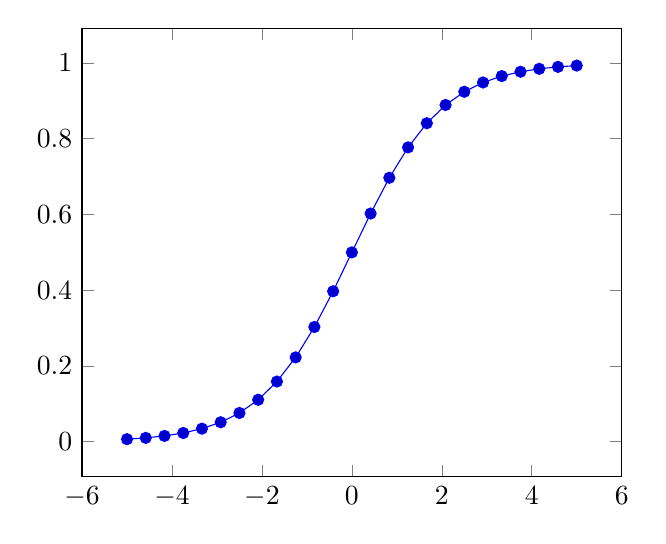
\begin{tikzpicture}
	\begin{axis}

		\addplot expression { 1/(1+exp(-x) };

	\end{axis}
	\end{tikzpicture}
	}
	\caption{Sigmoide Aktivierungsfunktion}
	\label{fig:Sigmoide Aktivierungsfunktion}
\end{figure}
	\item \textit{tf.relu} ersetzt mittlerweile immer mehr die Sigmoide Version. 
	Ein Grund dafür ist, dass die Berechnung mit Sigmoidefunktionen Ressourcen intensive ist. 
	Die rektifiziert lineare Funktion ist sehr viel einfacher, denn Werte unter $0$ werden als $0$ weiter gegeben und Werte darüber linear. 
	Somit resultiert ein Eingangswert von $-0.1$ in einer $0$ und ein Wert von $0.5$ in $0.5$.
	Wie im Diagramm \ref{fig:rektifiziert lineare Aktivierungsfunktion} ersichtlich ist, führt dies bei einem negativen Wert dazu, dass eine Multiplikation mit der Gewichtung in der nächsten Ebene ebenfalls in einer $0$ sich repräsentiert und somit in der Addition ignoriert wird.
\begin{figure}
	\centering
	\resizebox {\linewidth} {5cm} {
	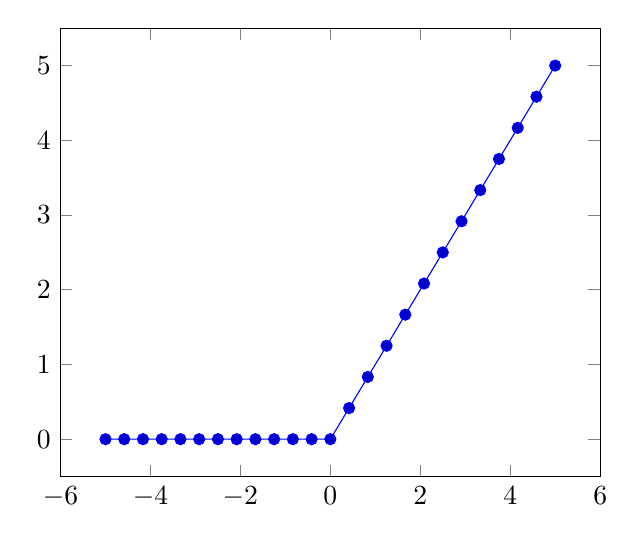
\begin{tikzpicture}
	\begin{axis}

		\addplot expression { max(0, x)};

	\end{axis}
	\end{tikzpicture}
	}
	\caption{rektifiziert lineare Aktivierungsfunktion}
	\label{fig:rektifiziert lineare Aktivierungsfunktion}
\end{figure}
	\item \textit{tf.tanh} genannt als Hyperbolic Tangent gehört ebenfalls zu den grundlegenden Aktivierungsfunktionen. 
	Der Unterschied zwischen dieser Funktion und der Sigmoiden Aktivierungsfunktion ist, dass der untere Grenzwert nicht bei $0$ liegt sondern bei $-1$. 
	Im Diagramm \ref{fig:Hyperbolic Tangents Aktivierungsfunktion} ist zu sehen, wo sich der Wendepunkt befindet, was im Falle des Hyperbolic Tangent in der Koordinate $x = 0, y = 0$ ist. 
\begin{figure}
	\centering
	\resizebox {\linewidth} {5cm} {
	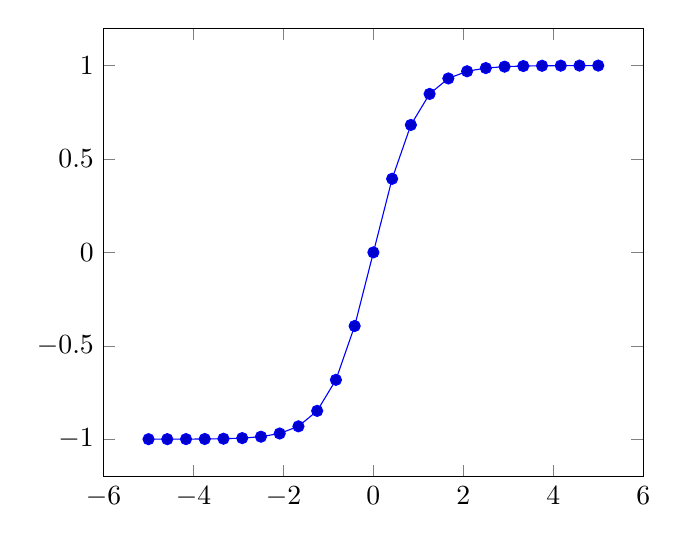
\begin{tikzpicture}
	\begin{axis}

		\addplot expression { tanh(x)};

	\end{axis}
	\end{tikzpicture}
	}
	\caption{Hyperbolic Tangents Aktivierungsfunktion}
	\label{fig:Hyperbolic Tangents Aktivierungsfunktion}
\end{figure}
\end{itemize}
Zu diesen Aktivierungsfunktion stehen noch einige weiter zur Verfügung, die ausführlich getestet gehören. 
Im Grunde könnte jede Funktion verwendet werden, doch jede besitzt eine Eigenheit und beeinflusst so den gesamten Graphen. 

\paragraph{Faltung Operationen} werden bei Bilderkennungen unter anderem deshalb verwendet, da sie eine Operation auf einen Stapel an Daten gleichzeitig anwenden. 
So wird wird ein Fenster über ein Bild geschoben und auf jedes Bild wird in dem selben Fenster die Operation durchgeführt. 
Diese Operation generalisiert die darunterliegenden Daten, so als ob sie auf Etwas reagiert hätten. 
Dies entspricht dem als ob ein Auge auf etwas reagiert hätte. 
\textbf{TODO: Diagramm}
\begin{itemize}
	\item \textit{tf.nn.conv2d} steht für zweidimensionale Bilder zur Verfügung. 
	\item \textit{tf.nn.conv3d} ermöglicht es mit dreidimensionale Objekte zu arbeiten.
\end{itemize}
Des Weiteren stehen noch weitere spezialisierte Versionen implementiert zur Verfügung.

\paragraph{Bündelung} wird verwendet um Daten zu vereinfachen. 
Eine Faltungsoperation führt dazu, dass aus einem Bild viel erzeugt werden mit unterschiedlichen Filtern. 
Eine Bündelung ermöglicht einen Vereinfachung der Bilder, sodass sie vereinfacht werden und dabei die Schlüsselinformationen aber dennoch erhalten bleiben. 
Diese Technik wurde zu früheren Zeiten eingesetzt, um Computerressourcen zu sparen, da diese nicht so leistungsfähig waren wie sie aktuell sind. 
TensorFlow bietet mehrere Umsetzungen, so kann der Maximalwert aus der Filtermatrix übernommen werden wie aber auch der Mittelwert. 

\paragraph{Verluste} beschreiben wie sehr ein Ergebnis von dem erwarten Ergebnis entfernt ist. 
Diese Art der Verlust Feststellung wird bei Regression Probleme benötigt aber auch regulieren im generellen.
\begin{itemize}
	\item \textit{tf.nn.l2\_loss} berechnet einen Wert, welcher den Inhalt des Tensors repräsentiert. 
	Im Falle dieser Implementierung wird keine Wurzel des Quadrats berechnet, sondern es werden die Werte nur addiert und durch $2$ dividiert.
	\item \textit{tf.nn.log\_poisson\_loss} berechnet den Logarithmischen-Wahrscheinlichkeitsverlust zwischen einem Ergebnis und einem erwarteten Ergebnis. 
	Diese Methode liefert im Normalfall nicht den exakten Verlust, was für Optimierungen nicht das Problem ist. 
	Sollte trotzdem ein genaueren Wert berechnet werden zum Vergleichen von Verlusten, muss die aufwändige Stirling Approximation aktiviert werden. 
\end{itemize}

\paragraph{Klassifizierungen} repräsentieren eine großen Bereich des maschinellen Lernens. 
TensorFlow besitzt deshalb mehrere Hilfsfunktionen, welche das arbeiten mit Klassifizierungen erleichtert. 
\begin{itemize}
	\item \textit{tf.nn.softmax} bildet alle Ergebnisse auf einen prozentualen Bereich ab. 
	So ergeben alle möglichen Ausgänge in Summe 100\%, was soviel bedeutet das ein Ergebnis eine gewisse Wahrscheinlichkeit besitzt. 
	\item \textit{tf.nn.softmax\_cross\_entropy\_with\_logits} bietet einem die Möglichkeit auf nicht skalierte Daten ein Ergebnis zu Berechnen, welches eine \textit{tf.nn.softmax} Berechnung liefern würde. 
	Zusätzlich wird eine weitere so genannte 'cross entropy' Operation ausgeführt, wo das Ergebnis für Optimierungen benötigt wird. 
	Die gesamte Methode berücksichtigt Spezialfälle im gesamten Prozess, welche schwer manuell ab zu berücksichtigen sind. 
\end{itemize}
\phantom \newline

\noindent
Zu diesen existieren noch weitere Implementierungen mit weiteren Eigenheiten, welche in diversen Situation möglicherweise einen Vorteil bieten. 

%\paragraph{Wiederkehrend Neuronale Netzwerke} 

\noindent
Des Weiteren gibt es Implementierungen für Wiederkehrende Neuronale Netzwere und weiter Dinge in diesem Themengebiet. 
\footnote{Online Dokumentation: Neural Network \url{www.tensorflow.org/api_guides/python/nn}}

\subsubsection{Running Graphs}

\paragraph{Session} stellt eine Hauptklasse des TensorFlow-Systems dar, mit der TensorFlow Engine im Hintergrund.
In ihr werden alle Operationen ausgeführt und alle Tensoren evaluiert. 
Dieser Session wird der Graphen mitgegeben, in dem der Endpunkt des Graphen angeben wird. 
Zur Ausführungszeit führt die Engine alle Operationen des Graphen durch und evaluiert die Tensoren in diesem. 
Die Engine führt dabei alles bis zu dem gegebenen Punkt aus, welcher als Ausgangspunkt übergeben wurde. 
Sollte der Graphen weiterführen, so wird dieser nicht mehr durchlaufen. 
Dies bietet eingeschränkte Möglichkeit, um das aufgebaute System zu testen. 
Eine Session wird mit \textit{tf.Session} erstellt und stellt die Funktionalität zum Ausführen, sowie die Möglichkeit diese zu schließe zur Verfügung. 
Mit \textit{tf.InteractiveSession} wird ebenfalls eine Session erstellt, diese wird aber zugleich als Basissession installiert. 
Dies bietet die Möglichkeit interaktive in einer Kommandozeile Operationen auszuführen, ohne die Session expliziert zu übertragen und anzusprechen. 
Die Tensoren und Operatoren bietet in diesen Fall die Option sich und den Graphen auszuführen, indem die Methoden \textit{TensorVariable.eval} sowie \textit{OperationsVariable.run} in diesen Aufgerufen werden. 

\noindent
Zusätzlich kann eine bestehende Basissession geholt werde sowie auf Fehler reagiert werden. 
\footnote{Online Dokumentation: Running Graphs \url{www.tensorflow.org/api_guides/python/client}}

\subsubsection{Training}

\paragraph{Optimizers} stellen einen weiteren Kernteil des System dar. 
TensorFlow stellt einen Menge an implementierten Optimierungsalgorithmen zur Verfügung. 
Diese Operationen trainieren den Graphen mit der gewählten Technik des gewählten Algorithmus. 
Diese Implementierungen versuchen die gegebenen Kosten eines Graphen zu minimieren. 
Bei der Verwendung von \textit{minimize} führt die Operation zwei Schritte in einem aus. 
In diesem wird der Gradient berechnet und dieser wird direkt auf die Variablen adaptiert. 
Diese Schritte können in einzelne zerlegt werden wenn, sollte mit den berechneten Gradient noch etwas zusätzlich durchgeführt werden. 
Die Berechnung wird dabei mit \textit{opt.compute\_gradients} ausgelöst, was einen Liste mit Paaren liefert. 
Diese Liste kann bearbeitet werden aber auch zu Testzwecken mit Protokolliert werden. 
Die Gradienten werden in dritten Schritt mit \textit{opt.apply\_gradients} auf die Variablen angewendet. 
Jeder Optimierungsalgorithmen verfügt über Eigenheiten und spezielle Verhalten, welche berücksichtigt werden sollten bei der Auswahl des Optimierers.

\paragraph{Gradient Computation} umfasst Methoden die das Verhalten des Graphen und der Optimierung beeinflussen. 
Diese Methoden ermöglichen es, Einfluss auf die Gradientenberechnung sowie auf dessen Evaluierung zunehmen. 
In diesem Sinne sind diese mit Vorsicht zu verwenden.

\paragraph{Verteilte Ausführung} stellt eine der Stärken von TensorFlow dar, da diese Technologie schon im System implementiert ist und somit keine manuelle Verteilung der Aufgaben entwickelt werden muss.
Dadurch besteht die Option die Berechnungen auf mehrere Geräte zu verteilen und so die zur Verfügung stehenden Ressourcen besser auszunützen. \\
%Im Grunde wird ein Cluster definiert welcher Computerknoten umfasst. 
%Diesen werden dann Tasks auf Aufgaben zugewiesen, wobei zu den Knoten definiert werden muss was zu tun ist.

\noindent
Einige Komfortmethoden ermöglichen es einfacher eine Session zu erstellen und alle Variablen zu initialisieren, sowie im Anschluss zu trainieren, wobei eine Stopbedingung mit definiert werden kann.
In diesem Zuge können Hooks einfach in das System integriert werden welche Aufgerufen werden.

\noindent
Im Weiteren kann Threading sowie der Verfall der Lernrate beeinflusst werden.
\footnote{Online Dokumentation: Training \url{www.tensorflow.org/api_guides/python/train}}

%\subsection{Probleme}

%\subsubsection{NaN Problem}

TensorFlow beinhaltet noch sehr viele weiter Komponenten und Möglichkeiten. 
Dies würde aber den Rahmen und den ersten Einblick in die Materie des maschinellen Lernens und im speziellen von TensorFlow sprengen. 
Im Grunde kann mit diesem Grundlagen und ein Netzwerk erstellt werden und damit gearbeitet werden. 
Seit der Offenlegung kommen immer mehr Erweiterungen aus der Community dazu, was auch dazu führt, dass Teile die sehr oft benötigt werden und aus mehreren Komponenten bestehen als Modul oder Funktion zur Verfügung stehen. 
Im Zuge dessen besteht die Möglichkeit sich einen bestehen Graphen zu nehmen, welcher zum Teil schon vor trainiert worden ist. 
Im Zuge dessen werden nur mehr die letzten Ebenen des Graphen trainiert und auf die konkrete Aufgabe hin ausgelegt. 
Dies hat zur Folge, dass schneller ein verwendbarer Graphen vorhanden ist, dieser aber sehr wahrscheinlich nicht der Beste ist den es geben würde. 

\subsection{TensorBoard}

TensorBoard stellt eine Erweiterung des TensorFlow-System dar, im Sinne einer Toolerweiterung. 
Jeder Graph kann in ein File Serialisiert werden, welches als Event-File bezeichnet wird. 
Dies hat zur Folge, dass dieser auch wieder geladen werden kann. 
Bei dieser Serialisierung werden alle Informationen des Graphen inklusive der Gewichtungen in die definierte Datei gespeichert.
TensorBoard bietet nun die Möglichkeit diesen Graphen zu laden und diesen Visualisiert darzustellen.
Zu den Graph-Informationen kann jeder Tensor mit gespeichert werden und als Diagramm visualisiert werden, mit einer zeitlichen Komponente. 
Dies ermöglicht es einem den Verlauf des Trainings zu analysieren. 
Aus einem Graphen können mehrere dieser Event-Files erzeugt werden sowie fixe Punkte definiert werden. 
Beim Laden eines Graphen in die TensorFlowt sowie TensorBoard-Umgebung kann spezifiziert werden zu welchen Zeitpunkt geladen werden soll. 
Damit wird ermöglicht viele Trainingsdurchläufe zu durchlaufen und bei einer Verschlechterung der Präzision zu einem früheren Zustand zurück zu springen.
Diese Tool ermöglichte es einem in das Verhalten eines Graphen ein wenig Einsicht zu nehmen und so die sogenannte Black Box zu durchleuchten. 

\paragraph{Namesbereiche (\textit{tf.name\_scope})} stellen eine Hilfe für die Darstellung und die Lesbarkeit des visualisierten Graphen dar. 
Durch die Verwendung des Python-Schlüsselwortes \textit{with} wird eine Ressource verwaltet und wieder freigegeben. 
In Verwendung mit \textit{tf.name\_scope} werden alle Operationen und Tensoren in diesem Block in der Visualisierung in einen benannten Block zusammengefasst.

\begin{figure}

\lstset{language=Python}
\begin{lstlisting}
import tensorflow as tf

with tf.name_scope("func"):
	b = tf.Variable(tf.zeros([100])) 
	W = tf.Variable(tf.random_uniform([784,100],-1,1)) 
	x = tf.placeholder(name="x") 
	relu = tf.nn.relu(tf.matmul(W, x) + b) 

C = [...] 
s = tf.Session()
for step in xrange(0, 10):
	input = ...construct 100-D input array ... 
	result = s.run(C, feed_dict={x: input}) 

	print step, result 
\end{lstlisting}

	\caption{TensorFlow Codefragment zur Namescope Verwendung in Graphen}
	\label{fig:NameScopeFragmentGraphDefinition}
\end{figure}
Wie in der Codefragment \ref{fig:NameScopeFragmentGraphDefinition} beschrieben werden die Tensoren und Operatoren \textit{b, W, x, relu} in einen Block zusammen gefasst. 
In diesem Beispiel gibt es keinen Tensor, welcher in den Block übergeben wird, da die Daten in der Ausführung von außerhalb es System in dieses gelangen. 
Die Operation \textit{relu} und der daraus resultierende Tensor bilden den Ausgang des Blockes. 
Diese Technik der Namensbereiche ermöglicht es einem den Graphen zu strukturiere, da nicht wie in \textit{tf.zeros([100])} viele einzelne Knoten dargestellt werden, sonder abstrahiert werden und aber weiterhin einsehbar sind.

\paragraph{Graph} bildet den Punkt zum Visualisieren des Graphen selbst. 
Hierbei werden aus dem Event-File alle Informationen zum Aufbau des Graphen geladen und visualisiert. 
Durch die Verwendung der Namensbereichen werden Gruppen gebildet was dazuführt, dass die Gruppierungen möglicherweise in Ebenen sich widerspiegeln. 
Der dargestellte Graphen kann nach dem Einlesen und generieren interaktive Analysiert werden. 
So können Bereiche vergrößert und geöffnet werden und die definierten Tensoren betrachtet werden. 
Dieses Tool bietet zusätzliche Funktionalitäten, wie das das Darstellen wo am meisten Rechenzeit benötigt wurde sowie auch welche Berechnung auf welchem Gerät ausgeführt worden ist. 
Alle diese zusätzlichen Funktionalitäten benötigen Daten, welchen beim Erstellen des Graphen mit definiert werden müssen und auch mit in des Event-File serialisiert werden müssen. 

\paragraph{Scalars} repräsentiert den Bereich, in welchem die Lernergebnisse dargestellt werden können. 
Dies umfasst die Präzision sowie die Verluste. 
Das Ziel des Graphen ist im Grunde immer die Präzision zu erhöhen und die Verluste zu minimieren. 
Aus diesem Grund sollte sich die Genauigkeit an $1$ annähern, außer die Definition dieser Berechnung liefert andere Werte oder besitzt einen anderen Grenzwert. 
Der Verlust sollte sich im laufe des Trainings an $0$ annähern, denn dadurch spiegelt sich die Fehlerquote ab. 
Dies hängt aber wieder von dem entwickelten Graphen ab und kann sich somit einem anderen Wert annähern.
\phantom \newline 

\noindent
Event bietet die Möglichkeit mehrere Graphen und ihre Eventdaten zu visualisieren. 
In diesem Fall werden alle gelesen Events in einer Liste aufgelistet, in welcher ausgewählt werden kann welche Ausführung in den Diagrammen dargestellt werden sollen. 
In diesem Zuge können diese Diagramme zusammen geführt werden und so die Ergebnisse direkt verglichen werden. 
Dies hat den Vorteil, dass ein Netzwerk mit Hyperparameter automatisch getestet werden kann und jede Kombination ein eigenes Event-File erzeugt. 
Solche Testdurchläufe benötigen mehr Zeit, abhängig von den definierten Kombinationen an Parameter, muss $x * y * ...$ alles durch getestet werden.
\phantom \newline

\noindent
Die Informationen für die Lernrate sowie des Verlustes werden in diesem Fall am besten Festgehalten. 
Dies wird ermöglicht indem die Tensoren, welche die Lernrate sowie den Verlust beinhalten, in die Methode \textit{tf.summary.scalar} jeweils gefüttert wird. 
Bei jedem Schreibzyklus in das Event-File werden diese Informationen dann mit übernommen und stehen dann in TensorBoard zur Verfügung.

\paragraph{Distributions} stellt eine weiter Funktionalität von TensorBoard dar.  %\url{https://duckduckgo.com/?q=tensorboard+histogram&ia=qa}
Diese Funktionalität war in den Versionen von 'r1.0' noch unter dem Punkt Histogramm. 
Im Allgemeinen werden Tensoren mit der Methode \textit{tf.summary.histogram} wieder das Event-File serialisiert. 
Das Ergebnis stellt einen Verteilung dar für die Werte die Tensor vorkommen. 
Dabei werden alle Werte auf eine Gaussian Glockenkurve projiziert. 
Das Diagramm repräsentiert auf der X-Achse die Anzahl der Schritte, die durchgeführt worden sind. 
Die Y-Achse gibt die konkreten Werte wieder, welche sich in dem Tensor über die Zeit befinden. 
\begin{figure}
	\centering
	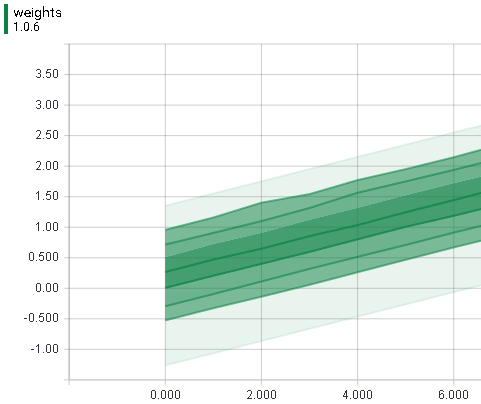
\includegraphics[scale=0.8]{images/Distripution-small.png}
	\caption{Verteilung der Werte in einem Tensor über die Zeit}
	\label{fig:Verteilungsdiagram}
\end{figure}
Im Diagramm \ref{fig:Verteilungsdiagram} wird ein Tensor mit 100 Werten dargestellt. 
Dieser Tensor wurde mit einer Normalverteilung initialisiert, wobei die Standartabweichung bei $0.5$ liegt und der Median zu Beginn bei $0.2$ liegt, mit einer geringen Abweichung. 
Die Linien in diesem Diagramm \ref{fig:Verteilungsdiagram} und ihre Einfärbungen präsentieren die Verteilung der Werte im beobachteten Tensor. 
Die Verteilung muss von unten Nach oben gelesen werden, dabei ergibt die unterste Linie den minimal Wert der vorgekommen ist. 
Die nächste Linie besagt, dass 7\% der Werte in dem Bereich zwischen dem geringsten und der zweiten Linie sich befinden, was inklusive des geringsten Wertes ist.  
Der nächste Bereich definiert, wie in einer Normalverteilung, dass bis zu Ende dieses Bereiches 16\% darin befinden. 
Im gesamten sind dies $9$ Markierungen mit 8 Bereichen, welche zusammen alle Werte im Tensor wieder spiegeln. 
Diese Folge an prozentualen Anteilen lauten wie folgend: $min, 7\%, 16\%, 31\%, 50\%, 69\%, 84\%, 93\%, max$. 
Im Diagramm \ref{fig:VerteilungsdiagrammPython} ist diese Verteilung besser ersichtlich, zusätzlich befinden sich in der Abbildung \ref{fig:Ergebnistensor} die Rohdaten der Diagramme. 
\begin{figure}
	\centering
	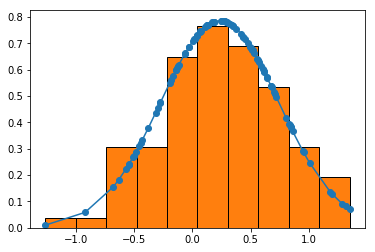
\includegraphics[scale=0.6]{images/gaussian.png}
	\caption{Verteilung der Werte in dem Tensor zu dem Diagramm \ref{fig:Verteilungsdiagram}}
	\label{fig:VerteilungsdiagrammPython}
\end{figure}
\begin{figure}

\lstset{language=Python}
\begin{lstlisting}
 -1.2645409,  -0.92252451, -0.68004417,  -0.63273954,  -0.57005012, 
 -0.5477351,  -0.54554129, -0.51146084,  -0.50482351,  -0.4872272, 
 -0.45631331, -0.44180638, -0.43258488,  -0.38066232,  -0.31675094, 
 -0.29567719, -0.27768314, -0.27437925,  -0.19503899,  -0.18343721, 
 -0.16653274, -0.13992153, -0.13946836,  -0.12969615,  -0.12044857, 
 -0.11908005, -0.06734778, -0.062724337, -0.032598898, -0.02885592, 
  0.006216079, 0.015204117, 0.018379062,  0.036883533,  0.041039094, 
  0.063002124, 0.068820029, 0.072805718,  0.11137276,   0.11735194, 
  0.12555882,  0.12613684,  0.13053563,   0.13633718,   0.17283598, 
  0.18271323,  0.18530971,  0.18671049,   0.24375655,   0.25207496, 
  0.27566099,  0.27588493,  0.27921408,   0.28581429,   0.29526407, 
  0.30613232,  0.32309669,  0.33705187,   0.34577289,   0.34687665, 
  0.37553167,  0.41834235,  0.43759531,   0.4376972,    0.45076531, 
  0.47984695,  0.49715465,  0.50634104,   0.51550949,   0.5168677, 
  0.53031796,  0.5579083,   0.56285316,   0.57165861,   0.59320259, 
  0.60513371,  0.61539149,  0.61814398,   0.63975775,   0.64333171, 
  0.67751783,  0.67795348,  0.68242437,   0.70252627,   0.70793462, 
  0.72128826,  0.80693412,  0.83029318,   0.83635086,   0.84400082, 
  0.84558558,  0.86151552,  0.95068389,   0.95598722,   1.0072051, 
  1.1837469,   1.1992682,   1.285683,     1.3168017,    1.3521272
\end{lstlisting}
	\caption{Sortierter Ergebnistensor zum Verteilungsdiagramm \ref{fig:VerteilungsdiagrammPython} und \ref{fig:Verteilungsdiagram} im Schritt $0$}
	\label{fig:Ergebnistensor}
\end{figure}


%[maximum, 93%, 84%, 69%, 50%, 31%, 16%, 7%, minimum]
%[maximum, μ+1.5σ, μ+σ, μ+0.5σ, μ, μ-0.5σ, μ-σ, μ-1.5σ, minimum]

%\textbf{TODO Grafik}

\paragraph{Histogram} passiert auf den selben Daten wie Verteilungsansicht. 
Im Grunde präsentiert diese Ansicht diese Daten nur auf eine andere Art und Weiße. 
\begin{figure}
	\centering
	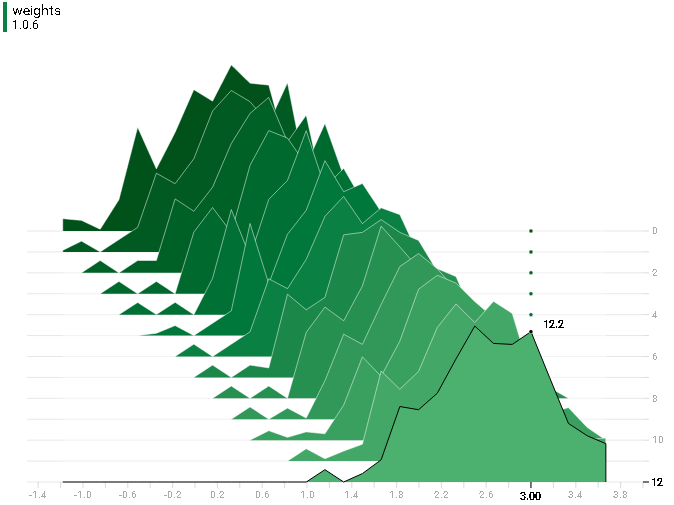
\includegraphics[scale=0.7]{images/histogram-value.png}
	\caption{Verteilung der Werte in dem Tensor in einem Histogramm}
	\label{fig:Histogram}
\end{figure}
Wie auch in der anderen Darstellung werden die Schritte, direkt auf einer Achse dargestellt. 
Im Falle des Histogramm \ref{fig:Histogram} ist dies die Achse, welche sich Dreidimensional aus dem Hintergrund des Bildes in den Vordergrund zieht. 
Die horizontalen Achsen welche zu jedem Schritt gezeichnet werden immer auf die vorderste Achse projiziert. 
Auf dieser wird der Wertebereich abgebildet, in welchem sich die Werte im Tensor befinden. 
Die Erhebungen und die sich darunter bildenden Flächen geben die Verteilung der Werte wieder. 
So wird beim überfahren eines Schrittes mit der Maus dieser aktiviert, wie im Histogramm \ref{fig:Histogram} ersichtlich ist. 
In Falle dieses Diagramms und dieser Stelle bedeutet dies, dass sich in der Nähe des Wertes $3.00$ ungefähr $12.2$ Einträge im Tensor befinden. 
Anders ausgedrückt haben $12.2$ konkrete Werte im Tensor den Wert $3.00$. 
Durch die Verteilung der Werte entsteht nun der Fall, das ein Teil der Einträge zu einem Wertebereich vorher oder nachher auch gehören können. 
Dieses Diagramm stellt die Verteilung in Wertebereiche dar, wobei alle vertikalen Werte in einem Schritt die Anzahl der Werte im Tensor ergeben müssen. 
Im Falle dieses Beispieles ergeben diese aufsummiert einen Wert von $100.044$, was gerundet die $100$ Einträge im Tensor bestätigt. 
Die Aufteilung der Werte in Wertebereiche mit teil Zuweisungen, erklärt auch den Schrittverlauf im Histogramm \ref{fig:Histogram}. 
Hier ist ersichtlich, dass sich die Verteilungen und Zugehörigkeiten immer ein wenig sich ändern, obwohl in diesem Beispiel in jedem Schritt konstant $0.2$ zu jedem Wert hinzu addiert worden ist. 
Dies lässt sich bei einer geringen Anzahl an Werten wie hier mit $100$ leichter beobachten, als bei einer sehr viel höheren. 
\phantom \newline

\noindent
Tensorboard bietet noch weiter Möglichkeiten, wie Bilder- oder Soundinhalte mit in das Event-File zu geben, um diese dann in Tensorboard weiter zu verwenden. 
So können diese Inhalte durch den Graphen gesendet werden und dabei beobachtet werden. 
Die letzte Erweiterung in Tensorboard ist der Punkt mit 'Emeddings', wo gelernte Informationen, so wie sie vom Graphen gruppiert worden sind, dargestellt werden können. \footnote{Online Dokumentation: Emeddings \url{www.tensorflow.org/get_started/embedding_viz}}
\phantom \newline

\noindent
Dieses Kapitel repräsentiert die grundsätzliche Funktionalität des TensorFlow-Systems. 
Es wurde auf die Grundlagen und die am Meist benötigten Methoden eingegangen. 
Das Verstehend dieser stellt die Grund für das nächste Kapitel dar. 
In diesem wird ein praktisches Beispiel mit TensorFlow erläutert. 








